\documentclass[12pt]{article}
\usepackage{amsmath, amssymb}
\usepackage{geometry}
\usepackage{hyperref}
\usepackage{tikz}
\usetikzlibrary{arrows.meta, decorations.markings}
\geometry{margin=1in}

\title{On the Nature of Mass II:\\
Local Constraint Generation and the Einstein Equations}
\author{Paul A. I. Reilly}
\date{[DRAFT v1.1 --- not for circulation]}

\begin{document}

\maketitle

%% ============================================================
\begin{abstract}
%% ============================================================

Building on Paper~I \cite{Reilly2026}, which derived the exterior
Schwarzschild metric from a local information generation hypothesis,
we derive the null--null components of Einstein's field equations
for vacuum and pressureless dust.
The central quantity is~$J$, the local rate density of irreversible
information generation, weighted by information content per outcome.
Infinitesimal causal diamonds serve as covariant local probes,
connecting null-boundary area growth to the bulk generation of
irreversible information \cite{Jacobson1995,Wald1984}.
In vacuum, $J=0$ and null-boundary area is conserved,
corresponding to the vacuum condition $R_{\mu\nu}=0$.
For dust, nonzero~$J$ drives local area growth.
Via the Raychaudhuri equation, this area growth determines
the null--null components of the Ricci tensor.
Expressing energy density directly in terms of~$J$,
and invoking Lovelock's theorem \cite{Lovelock1971} for the
unique divergence-free extension to a rank-2 tensor, yields
the Einstein equations as a local geometric consistency
condition: spacetime curvature is the accommodation that
geometry must make for irreversible information production.
The factor~$8\pi G$ emerges directly from the information--area
correspondence of Paper~I without appeal to a Newtonian limit.
This approach adopts Jacobson's \cite{Jacobson1995} use of
causal diamonds and the Raychaudhuri equation as local probes,
but replaces his thermodynamic input---the Clausius relation
applied to Rindler horizons---with the information generation
hypothesis, obtaining the field equations without invoking
temperature, entropy, or equilibrium conditions.
The cosmological constant is discussed but not derived;
its information-theoretic origin is deferred to the
companion paper on cosmology.
Extensions to pressure, shear, and general matter distributions
are discussed.

\end{abstract}

%% ============================================================
\section{Introduction}
%% ============================================================

\subsection{Relation to Paper~I}

In a companion paper \cite{Reilly2026} we showed that the exterior
Schwarzschild metric follows from a single hypothesis: an isolated
mass~$M$ of pressureless dust generates irreversible classical
information at the proper-time rate
\begin{equation}
  \frac{dC}{d\tau} = \frac{2\pi M c^2}{\hbar}, \label{eq:hypothesis}
\end{equation}
where~$C$ denotes accumulated irreducible classical information
in the sense of Kolmogorov \cite{Kolmogorov1965}, and the
factor~$2\pi$ is fixed by consistency with the Bekenstein bound
at the Compton scale.
Four assumptions governing the geometric accommodation of this
information---light-speed propagation~(A1), holographic saturation
of the vacuum near matter~(A2), the Bekenstein bound relating
information to area~(A3), and minimality~(A4)---suffice to derive
the radial Schwarzschild component~$g_{rr}$ without invoking
Einstein's field equations.
Assumption~A2 was adopted in Paper~I and validated a~posteriori
by the successful derivation of the correct metric.
Hypothesis~\eqref{eq:hypothesis} is stated for pressureless dust;
extensions to matter with pressure, shear, or momentum flux
are more complex and are addressed in the present and subsequent
companion papers.

The present paper extends this framework from a single spherically
symmetric mass to the local, covariant setting required for the
full Einstein equations.
Rather than asking what global geometry a given mass imposes on
its surroundings, we ask what geometry is required \emph{locally}
wherever irreversible information is being generated.
The answer, derived here for vacuum and pressureless dust,
is the null--null components of Einstein's field equations.

\subsection{The Central Quantity}

We quantify local information generation by~$J$, the
\emph{irreversible information generation rate density}:
the rate per unit proper volume at which irreversible classical
information is produced, weighted by information content per
outcome \cite{Shannon1948,Kolmogorov1965}.
The weighting is necessary because different physical outcomes
carry different amounts of information; a process that settles
a high-entropy question contributes more to local spacetime
geometry than one that settles a low-entropy question at the
same volumetric rate.
The precise definition and covariant transformation properties
of~$J$ are established in Section~\ref{sec:diamond}.

For pressureless dust with energy density~$\rho$ and
4-velocity~$u^\mu$, the mass in proper volume~$dV$ is
$dM = \rho\,dV/c^2$.
Applying hypothesis~\eqref{eq:hypothesis} per unit volume:
\begin{equation}
  J = \frac{dC/d\tau}{dV} = \frac{2\pi\rho}{\hbar}.
  \label{eq:J-dust}
\end{equation}
In vacuum, $J=0$: no irreversible processes occur, no new
classical information is generated, and null-boundary area
is conserved.
For dust, $J>0$: bulk information generation drives area growth
along null boundaries, and via the Raychaudhuri equation this
determines the null--null Ricci components.
Expressing energy density in terms of~$J$ then yields the
Einstein equations as a local consistency condition.

\subsection{Relation to Jacobson \cite{Jacobson1995}}

Jacobson showed that the full Einstein equations can be derived
by applying the Clausius relation $\delta Q = T\,dS$ to local
Rindler horizons, treating spacetime dynamics as equilibrium
thermodynamics \cite{Jacobson1995}.
This is a profound result.
The present approach borrows two pieces of Jacobson's
machinery---infinitesimal causal diamonds as covariant local
probes, and the Raychaudhuri equation connecting area growth
to Ricci curvature---but replaces his physical input entirely.
Where Jacobson requires the Clausius relation, the Unruh
temperature of an accelerated horizon, and the identification
of entropy with horizon area, the present derivation requires
only the information generation hypothesis~\eqref{eq:hypothesis}
of Paper~I.
No temperature is assigned to any surface.
No equilibrium condition is assumed.
The derivation is intrinsically non-equilibrium: irreversible
information generation is the input, and local curvature is
the output.

Causal diamonds are the natural covariant probes for this purpose.
Their null boundaries directly encode the light-speed propagation
of locally generated information established in Paper~I (A1),
and their infinitesimal limit provides the local geometric
language needed to translate a rate density~$J$ into a curvature
tensor component.

\subsection{Scope and Roadmap}

This paper derives the null--null Einstein equations for vacuum
and pressureless dust.
Pressure, shear, rotation, and the full stress-energy tensor
are deferred to companion papers.
The null--null components are the natural starting point:
they are the components probed by causal diamonds,
they capture the leading geometric response to energy density,
and the vacuum case $J=0$ provides a clean baseline.

Section~\ref{sec:diamond} defines~$J$ precisely and establishes
the causal diamond framework.
Section~\ref{sec:vacuum} treats vacuum: $J=0$, area conservation,
and the vacuum Ricci condition.
Section~\ref{sec:dust} treats dust: nonzero~$J$, the derivation
of area growth, and the null--null Einstein equations.
Section~\ref{sec:stress-energy} assembles the full Einstein tensor,
addresses the cosmological constant, and shows how~$8\pi G$
emerges from the information--area correspondence.
Section~\ref{sec:discussion} discusses implications, including
Newton's constant as a pixel-area conversion factor, the
connection to Paper~I's Schwarzschild derivation, and the
program for extending to general matter.

%% ============================================================
\section{The Causal Diamond Framework and the Definition of~$J$}
\label{sec:diamond}
%% ============================================================

\subsection{Infinitesimal Causal Diamonds}

Let $p$ be an event in spacetime.
Choose a null direction, specified by a future-pointing null
vector~$k^\mu$ at~$p$ with some convenient normalization.
The infinitesimal causal diamond associated with~$(p, k^\mu)$
is the intersection of the future light cone of a point~$p^-$
slightly to the past of~$p$ along~$k^\mu$ with the past light
cone of a point~$p^+$ slightly to the future, where the
affine separation is a small parameter~$\varepsilon$
(see Figure~\ref{fig:diamond}).
The diamond is small enough that higher-order curvature
corrections are negligible; we work throughout to leading
order in~$\varepsilon$.

We consider all possible orientations of the diamond---all
null directions~$k^\mu$ at~$p$---so that~$k^\mu$ is treated
as arbitrary.
This is essential: only by demanding that the geometric
condition hold for \emph{all} null~$k^\mu$ can we recover
the full tensor equation $R_{\mu\nu}=0$ or
$G_{\mu\nu}=8\pi G\,T_{\mu\nu}$ from its null--null
projections.

Let $A(\lambda)$ denote the cross-sectional area of the null
boundary at affine parameter~$\lambda$ along the null generators,
with $\lambda=0$ at the waist of the diamond.
The expansion scalar of the null congruence is
\begin{equation}
  \theta = \frac{1}{A}\frac{dA}{d\lambda}. \label{eq:expansion}
\end{equation}
The null boundaries of a causal diamond are hypersurface-orthogonal
by construction: the null generators are orthogonal to the
$(n{-}2)$-dimensional cross-sections $A(\lambda)$.
By the Frobenius theorem, hypersurface-orthogonality is equivalent
to vanishing twist: $\omega_{\mu\nu}=0$ exactly.

\begin{figure}[h]
\centering
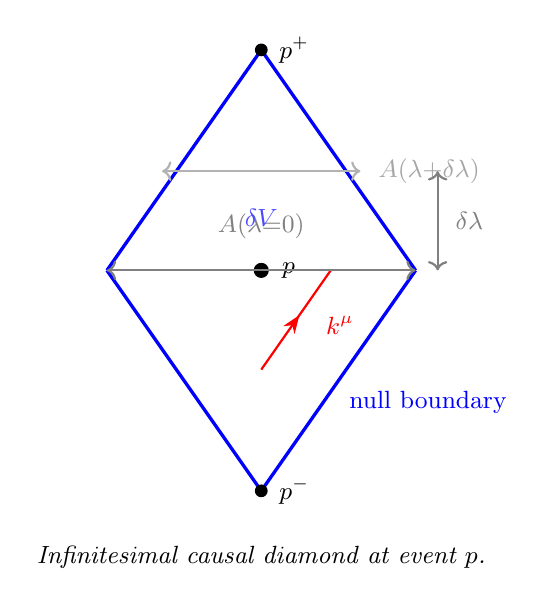
\begin{tikzpicture}[scale=1.4,
  nullray/.style={thick, postaction={decorate,
    decoration={markings, mark=at position 0.55 with {\arrow{Stealth}}}}},
  boundary/.style={very thick, blue},
  label/.style={font=\small}
]

%% --- diamond vertices ---
\coordinate (bottom) at (0,-2);
\coordinate (top)    at (0, 2);
\coordinate (left)   at (-1.4, 0);
\coordinate (right)  at ( 1.4, 0);

%% --- null boundaries (four edges of diamond) ---
\draw[boundary] (bottom) -- (right) node[midway, below right, label]
  {null boundary};
\draw[boundary] (bottom) -- (left);
\draw[boundary] (top)    -- (right);
\draw[boundary] (top)    -- (left);

%% --- central event p ---
\filldraw[black] (0,0) circle (1.8pt);
\node[label, right=4pt] at (0,0) {$p$};

%% --- null direction k^mu (upward along right edge) ---
\draw[nullray, red] (0,-0.9) -- (0.63, 0);
\node[label, red, right=2pt] at (0.45,-0.5) {$k^\mu$};

%% --- affine parameter labels along right boundary ---
\node[label, right=3pt] at (0,-2)   {$p^-$};
\node[label, right=3pt] at (0, 2)   {$p^+$};

%% --- cross-sectional area A(lambda) at waist ---
\draw[thick, <->, gray] (-1.4,0) -- (1.4,0);
\node[label, gray, above=3pt] at (0, 0.12) {$A(\lambda{=}0)$};

%% --- cross-sectional area at lambda = +delta lambda ---
\draw[thick, <->, gray!60] (-0.9, 0.9) -- (0.9, 0.9);
\node[label, gray!70, right=3pt] at (0.9, 0.9)
  {$A(\lambda{+}\delta\lambda)$};

%% --- delta lambda brace ---
\draw[thick, gray, <->] (1.6, 0) -- (1.6, 0.9);
\node[label, gray, right=3pt] at (1.6, 0.45) {$\delta\lambda$};

%% --- delta V label inside diamond ---
\node[label, blue!70] at (0, 0.48) {$\delta V$};

%% --- p- and p+ labels ---
\filldraw[black] (0,-2) circle (1.5pt);
\filldraw[black] (0, 2) circle (1.5pt);

%% --- caption note ---
\node[label, align=center] at (0,-2.6)
  {\textit{Infinitesimal causal diamond at event $p$.}};

\end{tikzpicture}
\caption{An infinitesimal causal diamond centered on event~$p$,
  bounded by past and future null cones from~$p^-$ and~$p^+$
  respectively.
  The null vector~$k^\mu$ is tangent to the null generators.
  The cross-sectional area~$A(\lambda)$ of the null boundary
  is measured at affine parameter~$\lambda$; the waist area
  $A(0)$ is shown at~$p$.
  The proper spatial volume~$\delta V$ of the interior and the
  affine thickness~$\delta\lambda$ are indicated.
  In vacuum ($J=0$): $A_{\rm out} = A_{\rm in}$, $\theta=0$,
  $R_{\mu\nu}k^\mu k^\nu = 0$.
  In dust ($J>0$): $A_{\rm out} > A_{\rm in}$,
  $R_{\mu\nu}k^\mu k^\nu = 4G\,J > 0$.}
\label{fig:diamond}
\end{figure}

\subsection{Definition of $J$}

The irreversible information generation rate density~$J$ at
event~$p$ is defined as follows.
Consider a small proper 4-volume~$\delta\Omega$ centered on~$p$.
Let $\delta C$ be the total irreducible classical information
(in the sense of Kolmogorov \cite{Kolmogorov1965}) generated
by irreversible R-processes within~$\delta\Omega$ during proper
time~$\delta\tau$, weighted by the information content per
outcome (in the sense of Shannon \cite{Shannon1948}).
Then
\begin{equation}
  J(p) = \lim_{\delta\Omega\to 0}
  \frac{\delta C}{\delta\Omega\,\delta\tau}. \label{eq:J-def}
\end{equation}
Since $\delta C$ is a scalar count of irreversible outcomes
and $\delta\Omega\,\delta\tau$ is a proper 4-volume element,
$J$ transforms as a Lorentz scalar under local changes of frame.
In vacuum, $J=0$ everywhere by definition: no irreversible
transitions occur and no new classical information is produced.
For dust at rest with energy density~$\rho$,
equation~\eqref{eq:J-dust} gives $J = 2\pi\rho/\hbar$.

%% ============================================================
\section{Vacuum Case}
\label{sec:vacuum}
%% ============================================================

\subsection{Area Conservation from $J=0$}

In Paper~I, assumption~A2 states that the vacuum near matter
operates at holographic saturation: newly generated information
requires a corresponding increase in bounding area.
The null boundary of a causal diamond encodes the information
content of its bulk interior.
If $J=0$ throughout a vacuum region---not merely at the center
of one diamond, but everywhere in the region containing~$p$---then
no new information is generated in any bulk, no new boundary area
is required, and the null-boundary area is conserved along
every null congruence in the region:
\begin{equation}
  \frac{dA}{d\lambda} = 0
  \quad\Longrightarrow\quad
  \theta = 0
  \quad \text{everywhere in the vacuum region.}
  \label{eq:vacuum-conservation}
\end{equation}
Since $\theta=0$ holds identically as a function of~$\lambda$,
differentiation gives
\begin{equation}
  \frac{d\theta}{d\lambda} = 0. \label{eq:vacuum-dtheta}
\end{equation}
This is the key step: area conservation in vacuum is not a new
postulate but a consequence of $J=0$ together with~A2
from Paper~I, which was itself validated by the successful
Schwarzschild derivation.

\subsection{The Raychaudhuri Equation}

The Raychaudhuri equation for a null congruence with
tangent~$k^\mu$ is \cite{Wald1984}
\begin{equation}
  \frac{d\theta}{d\lambda}
  = -\frac{1}{2}\theta^2
    - \sigma_{\mu\nu}\sigma^{\mu\nu}
    + \omega_{\mu\nu}\omega^{\mu\nu}
    - R_{\mu\nu}k^\mu k^\nu,
  \label{eq:raychaudhuri}
\end{equation}
where $\sigma_{\mu\nu}$ is the shear and $\omega_{\mu\nu}$
is the twist.
As established in Section~\ref{sec:diamond}, the twist vanishes
exactly for the hypersurface-orthogonal congruences of causal
diamonds: $\omega_{\mu\nu}=0$.
The shear $\sigma_{\mu\nu}$ accumulates from tidal distortions
of the congruence; in the infinitesimal diamond of size~$\varepsilon$,
a leading-order expansion of the geodesic deviation equation shows
$\sigma_{\mu\nu}=O(\varepsilon)$, so
$\sigma_{\mu\nu}\sigma^{\mu\nu}=O(\varepsilon^2)$
and is negligible at leading order.
This is the same approximation used by Jacobson~\cite{Jacobson1995}
and is standard in the infinitesimal causal diamond literature.

Substituting $\theta=0$, $d\theta/d\lambda=0$, $\omega_{\mu\nu}=0$,
and $\sigma_{\mu\nu}\sigma^{\mu\nu}\to 0$:
\begin{equation}
  0 = -R_{\mu\nu}k^\mu k^\nu,
  \qquad\text{i.e.,}\qquad
  R_{\mu\nu}k^\mu k^\nu = 0. \label{eq:null-null-vacuum}
\end{equation}

\subsection{Recovery of $R_{\mu\nu}=0$}

Equation~\eqref{eq:null-null-vacuum} holds for the
arbitrary null vector~$k^\mu$ at~$p$.
We recover the full vacuum condition using the following
algebraic lemma: if a symmetric tensor~$T_{\mu\nu}$ satisfies
$T_{\mu\nu}k^\mu k^\nu=0$ for all null~$k^\mu$, then
$T_{\mu\nu}=0$.
Proof: for any two null vectors~$k^\mu$ and~$l^\mu$,
expand $T_{\mu\nu}(k+l)^\mu(k+l)^\nu=0$ to obtain
$2T_{\mu\nu}k^\mu l^\nu=0$;
since every tangent vector can be written as a sum of null
vectors, all components of~$T_{\mu\nu}$ vanish
(see Wald \cite{Wald1984}, Appendix~B).
Applying this to $T_{\mu\nu}=R_{\mu\nu}$:
\begin{equation}
  R_{\mu\nu} = 0. \label{eq:vacuum-einstein}
\end{equation}
This is the vacuum Einstein equation, derived without invoking
the Einstein field equations, without thermodynamic input,
and without any assumption about entropy or temperature.
The vanishing of Ricci curvature in vacuum is the geometric
statement that no irreversible information is being generated
locally: $J=0 \Rightarrow R_{\mu\nu}=0$.

%% ============================================================
\section{Dust Case}
\label{sec:dust}
%% ============================================================

\subsection{Area Growth from Local Information Generation}

We now consider an infinitesimal causal diamond centered on an
event~$p$ within a distribution of pressureless dust.
The dust generates irreversible information at local rate
density~$J>0$, given by equation~\eqref{eq:J-dust}.
By assumption~A2 of Paper~I, each nat of information requires
a corresponding area increase of~$4\ell_P^2$ (assumption~A3),
where $\ell_P^2 = G\hbar/c^3$ is the squared Planck length.
By assumption~A1, this information propagates outward at~$c$,
so information generated within the diamond reaches the null
boundary during the affine interval~$\delta\lambda$.

The total irreversible information generated within the diamond
during affine interval~$\delta\lambda$ is
\begin{equation}
  \delta C = J\,\delta V\,\delta\lambda,
  \label{eq:deltaC}
\end{equation}
where $\delta V$ is the proper spatial volume of the diamond's
cross-section.
By assumptions~A2 and~A3, this information requires a
corresponding area increase on the null boundary:
\begin{equation}
  \delta A = 4\ell_P^2\,\delta C
           = 4\ell_P^2\,J\,\delta V\,\delta\lambda
           = \frac{4G\hbar}{c^3}\,J\,\delta V\,\delta\lambda.
  \label{eq:deltaA-full}
\end{equation}
In natural units ($\hbar=c=1$) this becomes
\begin{equation}
  A_{\rm out} - A_{\rm in}
  = 4G\,J\,\delta V\,\delta\lambda.
  \label{eq:area-growth}
\end{equation}
This is not an asserted scaling relation: the coefficient~$4G$
follows directly from the Bekenstein conversion (A3) applied
locally, with no free parameter.
The factor of~$4$ is Bekenstein's; the factor of~$G$ converts
information (in nats) to geometric area.
Newton's constant~$G$ plays the role of a pixel-area
conversion factor: $4G$ is the area of one information pixel
on a holographic screen, consistent with the interpretation
developed in Paper~I.

\subsection{Raychaudhuri and the Ricci Components}

From equation~\eqref{eq:area-growth}, the area growth per
unit affine parameter is
\begin{equation}
  \frac{dA}{d\lambda} = 4G\,J\,\delta V > 0.
  \label{eq:dA-dlambda}
\end{equation}
Dividing by~$A$, the expansion is
\begin{equation}
  \theta = \frac{1}{A}\frac{dA}{d\lambda}
         = \frac{4G\,J\,\delta V}{A}.
  \label{eq:theta-dust}
\end{equation}
For an infinitesimal diamond, $\delta V/A = O(\varepsilon)$, so
$\theta = O(\varepsilon)$ and the $\theta^2$ term in
Raychaudhuri~\eqref{eq:raychaudhuri} is $O(\varepsilon^2)$
and negligible at leading order.
Differentiating~\eqref{eq:theta-dust} with respect to~$\lambda$
and applying the same leading-order approximation
(dropping $\theta^2$ and $\sigma_{\mu\nu}\sigma^{\mu\nu}$,
setting $\omega_{\mu\nu}=0$), the Raychaudhuri equation gives
\begin{equation}
  R_{\mu\nu}k^\mu k^\nu
  = -\frac{d\theta}{d\lambda}
  = -\frac{d}{d\lambda}\!\left(\frac{4G\,J\,\delta V}{A}\right).
  \label{eq:ricci-intermediate}
\end{equation}
In the limit of the infinitesimal diamond, the ratio
$\delta V / A \to \delta\lambda$.
To see this geometrically: the cross-sectional area $A(\lambda)$
of the null boundary scales as $A \sim \varepsilon^2$ (two transverse
directions, each of size~$\varepsilon$), while the proper spatial
volume of the diamond's waist region scales as
$\delta V \sim \varepsilon^2 \cdot \delta\lambda$ (the two transverse
dimensions times the affine thickness).
Therefore $\delta V / A \sim \delta\lambda$, with the proportionality
constant approaching unity in the infinitesimal limit.
To leading order:
\begin{equation}
  \frac{d}{d\lambda}\!\left(\frac{4G\,J\,\delta V}{A}\right)
  = 4G\,\frac{dJ}{d\lambda}\,\delta\lambda
  + 4G\,J\frac{d(\delta V/A)}{d\lambda}.
\end{equation}
The second term involves $d(\delta V/A)/d\lambda$, which
is itself $O(\varepsilon)$ and contributes only at higher order.
At leading order:
\begin{equation}
  R_{\mu\nu}k^\mu k^\nu
  = 4G\,J.
  \label{eq:ricci-j}
\end{equation}
Equation~\eqref{eq:ricci-j} is the central result of this section:
the null--null Ricci component equals $4G$ times the local
irreversible information generation rate density.
The coefficient~$4G$ is not a fitting parameter; it is the
Bekenstein pixel area from~A3.

\subsection{Recovery of the Null--Null Einstein Equation for Dust}

For pressureless dust with energy density~$\rho$ and
4-velocity~$u^\mu$, substituting
$J = 2\pi\rho/\hbar$ (equation~\eqref{eq:J-dust}):
\begin{equation}
  R_{\mu\nu}k^\mu k^\nu
  = 4G \cdot \frac{2\pi\rho}{\hbar}
  = \frac{8\pi G\rho}{\hbar}.
  \label{eq:ricci-dust}
\end{equation}
The stress-energy tensor for dust is
$T_{\mu\nu} = \rho\,u_\mu u_\nu$.
The null--null component (contracting with~$k^\mu k^\nu$ for
a null vector~$k^\mu$ co-moving with the dust, so that
$u_\mu k^\mu = -E/c$ for energy~$E$) gives
$T_{\mu\nu}k^\mu k^\nu = \rho(u_\mu k^\mu)^2$.
In natural units, for a null vector normalized so that
$u_\mu k^\mu = 1$:
\begin{equation}
  T_{\mu\nu}k^\mu k^\nu = \rho.
  \label{eq:tmunu-null}
\end{equation}
This normalization $u_\mu k^\mu = 1$ is a convenient affine
parametrization choice, not a physical constraint.
The factor $8\pi G$ in the final result is independent of this
choice: rescaling $k^\mu \to \lambda k^\mu$ rescales both sides
of~\eqref{eq:ricci-tmunu} by $\lambda^2$ and leaves the equation
unchanged.
Therefore
\begin{equation}
  R_{\mu\nu}k^\mu k^\nu = 8\pi G\,T_{\mu\nu}k^\mu k^\nu,
  \label{eq:ricci-tmunu}
\end{equation}
where the factor $8\pi G = 4G \times 2\pi$ has emerged
from two independent sources: $4G$ from the Bekenstein
pixel area (A3), and $2\pi$ from the information generation
constant~$\alpha$ of hypothesis~\eqref{eq:hypothesis} ---
the same~$\alpha=2\pi$ fixed in Paper~I.

%% ============================================================
\section{The Einstein Tensor and the Cosmological Constant}
\label{sec:stress-energy}
%% ============================================================

\subsection{From Null--Null Components to the Full Einstein Tensor}

Equation~\eqref{eq:ricci-tmunu} holds for all null~$k^\mu$ at~$p$
(since~$k^\mu$ was arbitrary throughout).
By the algebraic lemma stated in Section~\ref{sec:vacuum}
(Wald \cite{Wald1984}, Appendix~B), the null--null condition
for all null~$k^\mu$ implies the full tensor equation:
\begin{equation}
  R_{\mu\nu} = 8\pi G\,T_{\mu\nu}.
  \label{eq:ricci-full}
\end{equation}
Taking the trace: $R = 8\pi G\,T$, where $T = g^{\mu\nu}T_{\mu\nu}$.
For pressureless dust in its rest frame,
$T_{\mu\nu} = \rho\,u_\mu u_\nu$ gives
$T = -\rho$ (with signature $-+++$).
Forming the Einstein tensor
$G_{\mu\nu} = R_{\mu\nu} - \tfrac{1}{2}Rg_{\mu\nu}$:
\begin{equation}
  G_{\mu\nu}
  = R_{\mu\nu} - \frac{1}{2}Rg_{\mu\nu}
  = 8\pi G\,T_{\mu\nu} - \frac{1}{2}(8\pi G\,T)g_{\mu\nu}
  = 8\pi G\!\left(T_{\mu\nu} - \frac{1}{2}Tg_{\mu\nu}\right).
  \label{eq:einstein-intermediate}
\end{equation}
For dust, $T_{\mu\nu} - \tfrac{1}{2}Tg_{\mu\nu}
= \rho u_\mu u_\nu + \tfrac{1}{2}\rho g_{\mu\nu}$.
The combination on the right-hand side is not the
standard stress-energy tensor but differs from it by a term
proportional to the metric.
The resolution lies in Lovelock's theorem.

\subsection{Lovelock's Theorem and Uniqueness}

Lovelock's theorem \cite{Lovelock1971} states that in
four-dimensional spacetime, the unique symmetric,
divergence-free, rank-2 tensor constructed from the metric
and its first and second derivatives is
\begin{equation}
  H_{\mu\nu} = a\,G_{\mu\nu} + b\,g_{\mu\nu},
  \label{eq:lovelock}
\end{equation}
for real constants~$a$ and~$b$.
The Bianchi identity $\nabla_\mu G^{\mu\nu}=0$ and conservation
$\nabla_\mu T^{\mu\nu}=0$ together require that the left-hand
side of the field equation be of the form~\eqref{eq:lovelock}.
Matching to equation~\eqref{eq:ricci-tmunu} and its full tensor
extension uniquely determines~$a=1$, giving
\begin{equation}
  G_{\mu\nu} + \Lambda g_{\mu\nu} = 8\pi G\,T_{\mu\nu},
  \label{eq:einstein-lambda}
\end{equation}
where $\Lambda = b/a = b$ is an undetermined constant:
the cosmological constant.

\subsection{The Cosmological Constant}

The present derivation does not fix~$\Lambda$.
Setting $\Lambda=0$ recovers the standard Einstein equations
but is an additional assumption beyond what the information-theoretic
framework establishes here.
In the context of Screen Theory, the cosmological constant has
a natural candidate interpretation: it encodes the background
rate of irreversible information generation by the quantum vacuum
itself, independent of any classical matter distribution.
This interpretation, and its connection to the cosmological
constant problem, is developed in the companion paper on
cosmology.
For the purposes of this paper we note only that
$\Lambda=0$ is a separate assumption, and that the
information-theoretic framework does not require it.

\subsection{Emergence of $8\pi G$}

It is worth making explicit how $8\pi G$ emerges from the
framework with no free parameters.
From Paper~I: each nat of information requires area $4\ell_P^2 = 4G$
(in natural units), from the Bekenstein bound~(A3).
From hypothesis~\eqref{eq:hypothesis}: the generation rate
carries a factor~$2\pi$, fixed by the Bekenstein bound at
the Compton scale.
Therefore the proportionality constant between $R_{\mu\nu}k^\mu k^\nu$
and $T_{\mu\nu}k^\mu k^\nu$ is:
\begin{equation}
  4G \times \frac{2\pi}{\hbar}
  = \frac{8\pi G}{\hbar}
  \xrightarrow{\hbar=1} 8\pi G.
  \label{eq:8piG}
\end{equation}
The factor~$4G$ is one information pixel (Bekenstein);
the factor~$2\pi$ is the generation constant~$\alpha$ from
Paper~I.
Newton's constant~$G$ is the pixel-area conversion factor:
it is not a fundamental coupling but the exchange rate between
one nat of information and the minimum area required to
express it physically, up to the factor of~4 from Bekenstein.

%% ============================================================
\section{Discussion and Conclusions}
\label{sec:discussion}
%% ============================================================

\subsection{Summary}

We have derived the null--null components of Einstein's field
equations for vacuum and pressureless dust directly from local
irreversible information generation, quantified by~$J$.
Using infinitesimal causal diamonds~\cite{Jacobson1995,Wald1984},
we related null-boundary area changes to~$J$, showing that
area conservation ($J=0$) corresponds to vacuum curvature
($R_{\mu\nu}=0$), while positive~$J$ produces expansion along
null directions with $R_{\mu\nu}k^\mu k^\nu = 4G\,J$.
Substituting $J=2\pi\rho/\hbar$ for dust yields
$R_{\mu\nu}k^\mu k^\nu = 8\pi G\,T_{\mu\nu}k^\mu k^\nu$.
Lovelock's theorem \cite{Lovelock1971} extends this to the
full Einstein tensor, with the cosmological constant remaining
as an undetermined constant not fixed by the present framework.

\subsection{Connection to Paper~I}

Paper~I derived the radial metric component~$g_{rr}$ from
a global information balance around a spherically symmetric
stationary mass.
The present paper provides an independent confirmation of
the same physical content: in the exterior vacuum region of
such a mass, $J=0$ and $R_{\mu\nu}=0$, consistent with the
Schwarzschild metric being Ricci flat in the exterior.
The two papers are telling the same story at different scales
and in different languages: Paper~I gives the global geometry
sourced by a localized mass, Paper~II gives the local condition
that geometry satisfies wherever~$J$ takes a given value.
The g_tt conjecture of Paper~I --- that A4 (minimality)
excludes all unsourced free parameters in the temporal metric
component --- is not resolved by the present derivation, though
the fact that $G_{\mu\nu}=8\pi G T_{\mu\nu}$ is established here
provides strong additional motivation for the conjecture.

\subsection{Newton's Constant as a Pixel-Area Conversion Factor}

The identification of~$G$ as a pixel-area conversion factor ---
$4G$ being the area of one information pixel --- gives Newton's
constant a precise information-theoretic meaning.
Its apparent smallness (in SI units) is not a mystery to be
explained by a hierarchy of scales; it is the ratio of two
independently motivated fundamental quantities: the Planck
area $\ell_P^2 = G\hbar/c^3$ and the quantum of action~$\hbar$.
The factor~$c^3$ adjusts units only.
This reinterpretation is consistent with the result of Paper~I
and does not require any modification of the quantitative
predictions of general relativity.

\subsection{Future Directions}

\begin{enumerate}
  \item \textbf{General matter distributions.}
        Incorporating pressure and shear requires generalizing
        the definition of~$J$ beyond~\eqref{eq:J-def} to account
        for momentum flux and anisotropic stress.
        The off-diagonal and spatial components of~$T_{\mu\nu}$
        require constraint generation processes with directional
        properties not present in pressureless dust.

  \item \textbf{Black holes and horizons.}
        The event horizon of a black hole is the surface where
        the information export rate equals the generation rate
        of the interior mass.
        The Bekenstein-Hawking entropy $S=A/4G$ counts queued
        information at the horizon; Hawking radiation is the
        slow publication of this queue.
        The Page curve and information paradox have natural
        restatements in this framework.

  \item \textbf{Cosmology.}
        The companion paper applies the framework to expanding
        spacetimes, where bulk information accumulation on
        cosmic horizons may drive large-scale curvature.
        The cosmological constant receives a natural candidate
        interpretation as the vacuum information generation rate.

  \item \textbf{Action principles.}
        Whether the Einstein--Hilbert action can be derived
        from an information-theoretic variational principle
        is an open question.
        The identification of $G$ as a pixel-area factor
        suggests the action integral may have a direct
        combinatorial interpretation.
\end{enumerate}

%% ============================================================
\section*{Acknowledgments}
%% ============================================================

The author thanks Joel Welling for illuminating early
conversations about the holographic principle.

%% ============================================================
\section*{References}
%% ============================================================

\begin{enumerate}

  \item\label{Reilly2026}
        Reilly, P.\,A.\,I.\ (2026).
        On the Nature of Mass: Complexity Generation and
        Spacetime Curvature. [Preprint, Paper~I in this series].

  \item\label{Jacobson1995}
        Jacobson, T.\ (1995).
        Thermodynamics of Spacetime: The Einstein Equation
        of State.
        \textit{Physical Review Letters}, 75, 1260--1263.

  \item\label{Wald1984}
        Wald, R.\,M.\ (1984).
        \textit{General Relativity}.
        University of Chicago Press.

  \item\label{Lovelock1971}
        Lovelock, D.\ (1971).
        The Einstein Tensor and Its Generalizations.
        \textit{Journal of Mathematical Physics}, 12, 498--501.

  \item\label{Shannon1948}
        Shannon, C.\,E.\ (1948).
        A Mathematical Theory of Communication.
        \textit{Bell System Technical Journal},
        27, 379--423 and 623--656.

  \item\label{Kolmogorov1965}
        Kolmogorov, A.\,N.\ (1965).
        Three Approaches to the Quantitative Definition
        of Information.
        \textit{Problems of Information Transmission},
        1(1), 1--7.

\end{enumerate}

\end{document}
